%%%%%%%% ICML 2026 EXAMPLE LATEX SUBMISSION FILE %%%%%%%%%%%%%%%%%

\documentclass{article}

% Recommended, but optional, packages for figures and better typesetting:
\usepackage{microtype}
\usepackage{graphicx}
\usepackage{subcaption}
\usepackage{booktabs} % for professional tables

% hyperref makes hyperlinks in the resulting PDF.
% If your build breaks (sometimes temporarily if a hyperlink spans a page)
% please comment out the following usepackage line and replace
% \usepackage{icml2026} with \usepackage[nohyperref]{icml2026} above.
\usepackage{hyperref}
\pdfstringdefDisableCommands{\def\\{ }}


% Attempt to make hyperref and algorithmic work together better:
\newcommand{\theHalgorithm}{\arabic{algorithm}}

% Use the following line for the initial blind version submitted for review:
\usepackage{icml2026}

% For preprint, use
% \usepackage[preprint]{icml2026}

% If accepted, instead use the following line for the camera-ready submission:
% \usepackage[accepted]{icml2026}

\usepackage{amsmath}
\usepackage{amssymb}
\usepackage{mathtools}
\usepackage{amsthm}


% if you use cleveref..
\usepackage[capitalize,noabbrev]{cleveref}

%%%%%%%%%%%%%%%%%%%%%%%%%%%%%%%%
% THEOREMS
%%%%%%%%%%%%%%%%%%%%%%%%%%%%%%%%
\theoremstyle{plain}
\newtheorem{theorem}{Theorem}[section]
\newtheorem{proposition}[theorem]{Proposition}
\newtheorem{lemma}[theorem]{Lemma}
\newtheorem{corollary}[theorem]{Corollary}
\theoremstyle{definition}
\newtheorem{definition}[theorem]{Definition}
\newtheorem{assumption}[theorem]{Assumption}
\theoremstyle{remark}
\newtheorem{remark}[theorem]{Remark}

% Todonotes is useful during development; simply uncomment the next line
%    and comment out the line below the next line to turn off comments
%\usepackage[disable,textsize=tiny]{todonotes}
% \usepackage[textsize=tiny]{todonotes}

%%%%%%%%%%%%%%%%%%%%%%%%%%%%%%%%%%%%%%%%%%%%%%%%%%%%%%%%%%%%%%%%%%%%%%%%%%%%%%%
% TODO (ICML submission checklist / guidelines)
% - Page limit: fit the main body to 8 pages for initial submission (excluding
%   references/appendix). Do not reduce margins or font sizes.
% - Double-blind: remove/anonymize acknowledgements, institutional identifiers,
%   and any links that reveal author identity (code/data/project pages).
% - If you cite your own work, write in third person (avoid "in our prior work").
% - Ensure figures/tables are readable in 10pt, with captions under figures and
%   above tables.
% - Make sure the final PDF uses embedded Type-1 fonts.
%%%%%%%%%%%%%%%%%%%%%%%%%%%%%%%%%%%%%%%%%%%%%%%%%%%%%%%%%%%%%%%%%%%%%%%%%%%%%%%

% This conditionally hides identifying URLs unless the [accepted] or
% [preprint] option is enabled (those options set \ificmlshowauthors true).
\newcommand{\maskclassrepolink}{%
  \ificmlshowauthors%
    \href{https://github.com/khazum/MaskClass}{https://github.com/khazum/MaskClass}%
  \else%
    \texttt{[link omitted for double-blind review]}%
  \fi%
}
\newcommand{\ccimputedatasetslink}{%
  \ificmlshowauthors%
    \url{https://github.com/khazum/ccImputeDatasets}%
  \else%
    \texttt{[link omitted for double-blind review]}%
  \fi%
}

\usepackage{enumitem}
\usepackage{placeins} % \FloatBarrier to keep floats close to where referenced
\setlist[enumerate]{nosep}
% Reduce badness warnings for tight two-column layout.
\emergencystretch=1em
% The \icmltitle you define below is probably too long as a header.
% Therefore, a short form for the running title is supplied here:
\icmltitlerunning{MaskClass: Scalable and Accurate Single-Cell RNA-seq Analysis}

\newenvironment{compitemize}
  {\begin{itemize}[noitemsep, topsep=0pt, parsep=0pt, partopsep=0pt]}
  {\end{itemize}}

\begin{document}
\raggedbottom

\twocolumn[
\icmltitle{\texorpdfstring{MaskClass: A Masked Denoising Autoencoder for Scalable and\\
  Accurate Single-Cell RNA-seq Analysis}{MaskClass: A Masked Denoising Autoencoder for Scalable and Accurate Single-Cell RNA-seq Analysis}}


  % It is OKAY to include author information, even for blind submissions: the
  % style file will automatically remove it for you unless you've provided
  % the [accepted] option to the icml2026 package.

  % List of affiliations: The first argument should be a (short) identifier you
  % will use later to specify author affiliations Academic affiliations
  % should list Department, University, City, Region, Country Industry
  % affiliations should list Company, City, Region, Country

  % You can specify symbols, otherwise they are numbered in order. Ideally, you
  % should not use this facility. Affiliations will be numbered in order of
  % appearance and this is the preferred way.
  \icmlsetsymbol{equal}{*}

  \begin{icmlauthorlist}
    \icmlauthor{Marcin Malec}{iu,crane}
    \icmlauthor{Mehmet Dalkilic}{iu}
    \icmlauthor{Hasan Kurban}{iu,hbku}
  \end{icmlauthorlist}

  \icmlaffiliation{iu}{Computer Science Department, Indiana University, Bloomington, IN, USA}
  \icmlaffiliation{crane}{Naval Surface Warfare Center, Crane Division, Crane, IN, USA}
  \icmlaffiliation{hbku}{College of Science and Engineering, Hamad Bin Khalifa University, Doha, Qatar}

  \icmlcorrespondingauthor{Marcin Malec}{mamalec@iu.edu}

  % You may provide any keywords that you find helpful for describing your
  % paper; these are used to populate the "keywords" metadata in the PDF but
  % will not be shown in the document
  \icmlkeywords{scRNA-seq, Transcriptomics, Masked Denoising Autoencoder, Imputation}

  \vskip 0.3in
]

% this must go after the closing bracket ] following \twocolumn[ ...

% This command actually creates the footnote in the first column listing the
% affiliations and the copyright notice. The command takes one argument, which
% is text to display at the start of the footnote. The \icmlEqualContribution
% command is standard text for equal contribution. Remove it (just {}) if you
% do not need this facility.

% Use ONE of the following lines. DO NOT remove the command.
% If you have no special notice, KEEP empty braces:
\begin{NoHyper}
\printAffiliationsAndNotice{}  % no special notice (required even if empty)
\end{NoHyper}
% Or, if applicable, use the standard equal contribution text:
% \printAffiliationsAndNotice{\icmlEqualContribution}

\begin{abstract}
%While DNA contains the blueprint of an organism, RNA is the conductor that orchestrates the expression of this blueprint across diverse cellular components; thus, understanding RNA expression holds the key to understanding complex biological systems. 
The emergence of numerous single-cell ribonucleic acid (RNA) sequencing (scRNA-seq) technologies and protocols over the past decade has enabled the study of RNA expression at single-cell resolution with improved accuracy and scalability, now handling gene expression data from hundreds of thousands to millions of cells. However, scRNA-seq data present analytical challenges, including data sparsity, technical noise, and batch effects, which complicate downstream analyses, such as cell clustering and differential expression analysis. To address these challenges, we introduce MaskClass, a masked denoising autoencoder that significantly improves data quality by selectively hiding parts of gene expression data, learning to reconstruct them while minimizing the impact of noisy dropout values, and using a separate process to recover biological zero-expression measurements. While we focus our primary evaluation on scRNA-seq data, the proposed approach is applicable to other high-dimensional, sparse, and noisy data modalities, including other single-cell omics proteomics, spatial transcriptomics, and related domains characterized by structured missing data and measurement noise. Benchmarking against state-of-the-art denoising methods demonstrates MaskClass's effectiveness in noise reduction on simulated data and significant improvement in cell identity clustering across diverse real-world datasets. MaskClass is available as an open source implementation at \maskclassrepolink.
\end{abstract}

\section{Introduction}
Single-cell RNA sequencing (scRNA-seq) technologies and protocols enable the measurement of RNA expression across individual cells, allowing the study of biological systems at a level of detail and scale previously unattainable, providing more insight into cellular function and response across a variety of contexts, such as disease vs. non-disease states or therapeutic drug response. As this technology continues to grow in scale, the issue of significant technical variation and noise, primarily resulting in sparse count matrices with numerous zeros, is compounded. This issue arises from the low capture efficiency and shallow sequencing depth of current droplet protocols \citep{Zheng2017TenX}, leading to many expressed genes recorded as zero -- a phenomenon known as "dropout" event. Notably, not all zeros in the data indicate missing values. True biological zeros coexist with false zeros. This phenomenon complicates downstream analyses such as trajectory inference, differential expression (DE) analyses, and clustering. Using naive imputation methods to impute dropout events can distort genuine differences between cell types or states \citep{Svensson2020NotZI,Jiang2022ZeroInflationReview}. Consequently, effective methods for denoising and imputation must balance three objectives: (i) recovering likely missing counts, (ii) preserving true biological variability, and (iii) computational scaling to accommodate datasets comprising hundreds of thousands or millions of cells per sample. In this study, we introduce MaskClass, a masked denoising autoencoder that randomly conceals subsets of gene–cell entries during training. This model learns to reconstruct hidden entries while intentionally disregarding noisy data to recover likely missing values without. We benchmark MaskClass against state-of-the-art denoising and imputation methods, including MAGIC (Markov Affinity‑based Graph Imputation of Cells) \citep{vanDijk2018MAGIC}, Single-cell Analysis Via Expression Recovery (SAVER) \citep{Huang2018SAVER}, scImpute \citep{Li2018scImpute}, Deep Count Autoencoder (DCA) \citep{Eraslan2019DCA}, ccImpute \citep{Malec2022ccImpute}, and AutoClass \citep{Li2022AutoClass}. These methods represent a range of complementary modeling approaches and are influential in advancing the field. However, we acknowledge that many additional techniques exist beyond the scope of this evaluation. MAGIC constructs a k-nearest-neighbor affinity graph in a reduced space (principal component analysis, PCA), normalizes it into a Markov transition matrix ($M$), and then raises $M$ to a power $t$ to diffuse information across neighborhoods; the final imputed matrix is $M^t X$, where $X$ is the original expression matrix. In benchmark datasets, MAGIC recovered gene–gene relationships and phenotypic continua that were obscured in the raw data and increased concordance with independent protein measurements \citep{Eraslan2019DCA}. However, diffusion necessarily modifies all entries, including values not affected by dropout, which can over-smooth if $t$ is not well-tuned \citep{Li2018scImpute,Malec2022ccImpute}. scImpute models the probability that a zero (or low count) is a dropout versus a true zero for each gene–cell pair by fitting a mixture model; it then imputes only entries with high dropout probability by borrowing information from similar cells identified using genes unlikely to be affected by dropout. This design explicitly aims to avoid altering unaffected measurements while improving the DE and clustering performance on simulated and real datasets. Related critiques note that methods that modify all values (e.g., global smoothing) may introduce bias or erase meaningful heterogeneity if they fail to distinguish between true and false zeroes \citep{Malec2022ccImpute,Jiang2022ZeroInflationReview}. Gene-aware Bayesian recovery, in tandem with cell-smoothing strategies, utilizes cross-gene information and uncertainty quantification. SAVER suggests that unique molecular identifier (UMI) counts for each gene in each cell follow a Poisson–Gamma (negative binomial) model, with prior parameters estimated via Poisson Lasso regression on other genes. This approach generates a posterior distribution (and mean) for the latent true expression, providing both point estimates and credible uncertainty intervals (UIs). SAVER has shown proficiency in recovering distributional properties (e.g., Gini coefficients) consistent with RNA FISH, restoring attenuated gene–gene correlations, and avoiding spurious correlations seen with certain graph-smoothing methods, while explicitly quantifying uncertainty for downstream analysis. The rise of deep learning has enabled the development of count-aware autoencoders that merge nonlinear representation learning with likelihood-based reconstructions. DCA replaces the mean squared error with a negative binomial (NB) or zero-inflated NB (ZINB) likelihood, learning gene-specific means and dispersions (and dropout probabilities) while compressing data through a bottleneck layer. This count-modeling loss is crucial because, unlike a standard autoencoder, DCA effectively recovers the cell type structure in simulations with significant dropout and scales linearly to millions of cells, making it attractive for modern atlas-scale datasets. DCA also highlights the distinction between true and false zeros and offers diagnostics to choose between the NB and ZINB models depending on the technology; notably, UMI-based droplet data often do not require zero-inflated models \citep{Eraslan2019DCA,Svensson2020NotZI}.  

Building on autoencoders, AutoClass enhances the bottleneck with a classifier branch trained on pseudo-labels derived from pre-clustering, fostering latent representations that maintain biologically relevant structures, whereas the autoencoder reduces the noise. Unlike distribution-specific methods, AutoClass is explicitly distribution-agnostic and addresses a wide range of noise sources (not just dropout), including amplification bias, library size variation, batch effects, and other non-signal variations. Across simulated and real datasets, the two-branch architecture improved data recovery, clustering, differential expression (DE), and batch correction, demonstrating robustness to the key hyperparameters. Finally, ccImpute represents a consensus clustering-based strategy designed to correct dropout data. Inspired by Single-Cell Consensus Clustering (SC3) \citep{Kiselev2017SC3}, ccImpute computes a cell–cell consensus similarity matrix and imputes likely dropouts by averaging the expression across reliably comparable cells. The authors stressed that imputation methods should minimize the introduction of new noise and avoid altering non-dropout values. They reported enhanced downstream clustering performance compared to several baselines on datasets with known cell identity. This study highlights the limitations of manifold diffusion methods, such as altering unaffected genes and failing to preserve true zeros, and advocates for consensus-based similarity as a stable foundation for imputation.

Collectively, these studies establish core principles for scRNA-seq recovery: leveraging shared structures among cells and genes, respecting the count nature of the data, avoiding erasing genuine heterogeneity, and, when feasible, quantifying uncertainty for downstream tasks \citep{Zheng2017TenX,Huang2018SAVER,Jiang2022ZeroInflationReview}. Building on this foundation, the present study introduces MaskClass, a masked, self-supervised denoising autoencoder that selectively hides parts of gene expression data and learns to reconstruct them. MaskClass aims to retain these advantages while further mitigating over-smoothing and zero-inflation artifacts, challenges that become increasingly significant as datasets expand in size and complexity.

\section{Methods}
\label{sec:methods}
\subsection{Experimental scRNA-seq Datasets}
We benchmarked the models using five publicly available scRNA-seq datasets, referenced by the first author of their originating publication: Blakeley~\cite{blakeley2015defining}, Pollen~\cite{pollen2014low}, Darmanis~\cite{darmanis2015survey}, Usoskin~\cite{usoskin2015unbiased}, and Li~\cite{li2017reference}. These datasets encompass a diverse range of biological origins and technical characteristics, as summarized in Table~\ref{tab:datasets}.

The confidence in the ground-truth labels varies across these datasets. The Blakeley, Li, and Pollen datasets provide high-fidelity labels derived from controlled experimental conditions and distinct cell lines. In contrast, Usoskin and Darmanis labels were assigned computationally via clustering and subsequent expert annotation. To ensure that the analysis focused on distinct cellular populations, cells annotated as "hybrids" in the Darmanis dataset were excluded.

We selected these datasets because they exhibit substantial sparsity and technical noise, making denoising and imputation challenging. In our experiments, we selected the top $1000$ highly variable genes (HVGs) using \texttt{scran} ~\cite{lun2016step}. Raw counts were library-size normalized by scaling each cell to the median library size and applying a $\log_2(1+\cdot)$ transform, yielding $\mathbf{X}_{\log}$. We retained genes expressed in at least three cells.

\begin{table*}[!ht]
\caption{Summary of the experimental scRNA-seq datasets used for benchmarking. $N$ denotes the number of samples (cells), $M$ the initial number of features (genes) prior to preprocessing, and $K$ the number of distinct cell clusters reported in the original study. Datasets are available at: \ccimputedatasetslink}
\label{tab:datasets}
\centering
\begin{tabular}{@{} l r r r l l @{}}
\toprule
\textbf{Dataset} & \textbf{N (Cells)} & \textbf{M (Genes)} & \textbf{K} & \textbf{Origin} & \textbf{Reference} \\
\midrule
Blakeley & 30 & 16,862 & 3 & Human blastocyst & \cite{blakeley2015defining} \\
Li & 561 & 55,186 & 7 & Human cell lines & \cite{li2017reference} \\
Pollen & 301 & 23,730 & 11 & Human cell lines & \cite{pollen2014low} \\
Darmanis & 420 & 21,516 & 8 & Human cortex & \cite{darmanis2015survey} \\
Usoskin & 622 & 19,532 & 4 & Mouse lumbar & \cite{usoskin2015unbiased} \\
\bottomrule
\end{tabular}
\end{table*}

\subsection{Synthetic Data Generation}
To assess the imputation accuracy against a known ground truth, we generated four synthetic datasets using the \textit{splatter} R package (v1.32.0)~\cite{zappia2017splatter}. Each simulation generated $M=1{,}100$ genes, and the probability of differential expression (likelihood of gene expression differing between cell groups) was set to $0.1$ (\texttt{de.prob = 0.1}).

To simulate technical noise, dropout midpoints and shapes were randomized per group or batch. We sampled
\texttt{dropout.\allowbreak mid} from [1,5] and \texttt{dropout.\allowbreak shape} from [-1.5,-0.5].
The datasets were designed with varying population structures:

\begin{compitemize}
  \item \textbf{Sim-Equal:} Two cell types, equal proportions (50\%, 50\%); dropout simulated per group.
  \item \textbf{Sim-Unequal:} Three cell types, unequal proportions (60\%, 30\%, 10\%); dropout simulated per group.
  \item \textbf{Sim-Rare:} Four cell types with a rare subpopulation (50\%, 25\%, 20\%, 5\%); dropout simulated per group.
  \item \textbf{Sim-Batch:} Three cell types (40\%, 30\%, 30\%) across three batches; dropout simulated per batch (\texttt{dropout.type="batch"}). TrueCounts were batch-effect-free (\texttt{batch.rmEffect=TRUE}); observed counts included batch effects and dropout.
\end{compitemize}

For each scenario we simulated multiple cell counts
$N\in\{1\mathrm{k},5\mathrm{k},10\mathrm{k},15\mathrm{k},20\mathrm{k},25\mathrm{k},50\mathrm{k},100\mathrm{k}\}$ ($\mathrm{k}=10^3$). Each simulation
provides a noisy observed count matrix \texttt{counts} and a ground-truth matrix
\texttt{TrueCounts}. Genes expressed in fewer than three cells were removed. We
library-size normalized both matrices by scaling each cell to the median library
size and applying $\log_2(1+\cdot)$, yielding \texttt{logcounts}
($\mathbf{X}_{\log}$) and \texttt{logTrueCounts} ($\mathbf{X}^{\star}_{\log}$).

\paragraph{Notation.}
Throughout, $\mathbf{X}_{\log}\in\mathbb{R}_{\ge 0}^{N\times G}$ denotes the
observed log-normalized matrix, $\mathbf{X}^{\star}_{\log}$ the corresponding
synthetic ground truth (when available), and $\mathbf{X}'_{\log}$ the
reconstructed matrix
produced by MaskClass. We write $x_{ij}$, $x^{\star}_{ij}$, and $x'_{ij}$ for
their respective entries. We denote the (unnormalized) count matrix by
$\mathbf{C}=\{c_{ij}\}$.

\subsection{Model Architecture}
MaskClass is a symmetric fully connected autoencoder with encoder
$f_\theta:\mathbb{R}^{G}\!\to\!\mathbb{R}^{d}$ and decoder
$g_\phi:\mathbb{R}^{d}\!\to\!\mathbb{R}^{G}$,
\[
\mathbf{h}_i=f_\theta(\tilde{\mathbf{s}}_i),\qquad
\hat{\mathbf{s}}_i=g_\phi(\mathbf{h}_i),
\]
where $\tilde{\mathbf{s}}_i$ is the corrupted, scaled input
(Sections~\ref{sec:scaling}--\ref{sec:masking}). The network uses one hidden
layer of width $64$ and a bottleneck $d{=}32$ with a symmetric decoder; each
block applies a linear transformation, followed by layer normalization and a
SiLU nonlinearity.
Let $\mathbf{S}=\mathrm{scale}(\mathbf{X}_{\log})$ and $\hat{\mathbf{S}}$ denote
the decoder outputs stacked across cells; reconstructions in log space are
obtained by inverse scaling, $\mathbf{X}'_{\log}=\mathrm{invscale}(\hat{\mathbf{S}})$.

\subsection{Gene Scaling}
\label{sec:scaling}
We apply a robust, monotone per-gene scaling with three steps:
\[
\begin{aligned}
\text{(Winsorize)}\quad &\bar{x}_{ij}=\min(\max(x_{ij},q^{(2)}_j),q^{(99.5)}_j),\\
\text{(Standardize)}\quad &z_{ij}=\frac{\bar{x}_{ij}-\mu_j}{\sigma_j},\qquad
\sigma_j\leftarrow\max(\sigma_j,\varepsilon),\\
\text{(Rescale)}\quad &s_{ij}=2\cdot\frac{z_{ij}-z^{\min}_j}{z^{\max}_j-z^{\min}_j}-1,\\
&\qquad z^{\max}_j-z^{\min}_j\ge\varepsilon.
\end{aligned}
\]
We denote the scaled matrix by $\mathbf{S}$ and use
$\mathrm{scale}(\cdot)$ / $\mathrm{invscale}(\cdot)$ for forward/inverse
transforms.
Here $\varepsilon>0$ is an arbitrary small constant used for numerical
stability (we use $\varepsilon=10^{-8}$).
We define $z^{\min}_j=\min_i z_{ij}$ and $z^{\max}_j=\max_i z_{ij}$.

\subsection{Masked Denoising Objective}
\label{sec:masking}
For each mini-batch $\mathcal{B}$ of cells, we sample a binary mask
$\mathbf{M}\!\in\!\{0,1\}^{|\mathcal{B}|\times G}$ with different rates for
zeros vs.\ non‑zeros in logcounts:
\[
\begin{aligned}
m_{ij}&\sim\mathrm{Bernoulli}(\pi_{ij}),\\
\pi_{ij}&=\begin{cases}
p_{\mathrm{zero}}p_{\mathrm{bio}}(i,j) & x_{ij}=0,\\
p_{\mathrm{nonzero}} & x_{ij}>0,
\end{cases}
\end{aligned}
\]
We use $(p_{\mathrm{zero}},p_{\mathrm{nonzero}})=(0.01,0.30)$ and fill masked
non‑zeros with zero in the scaled space.

\paragraph{Noise for masked zeros.}
For masked zero entries we inject noise (in log space) using the observed count
range per gene. Let $c_{ij}$ denote the (raw) count and
$c^{\max}_j=\max_i c_{ij}$.
\[
\begin{aligned}
\eta_{ij}&\sim\mathrm{Uniform}(0,\nu),\quad \nu=0.2,\\
\tilde{x}_{ij}&=\log_2(1+\eta_{ij}c^{\max}_j),
\end{aligned}
\]
then apply $\mathrm{scale}(\cdot)$.

\paragraph{Loss.}
Let $r_{ij}=\hat{s}_{ij}-s_{ij}$ denote the reconstruction residual in the
scaled space. For a mini-batch, let $\mathcal{Z}=\{(i,j): x_{ij}=0\}$ and
$\mathcal{N}=\{(i,j): x_{ij}>0\}$ denote observed zeros and non-zeros,
respectively. The weighted masked reconstruction loss is
\[
\mathcal{L}_{\mathrm{mask}}=
\frac{w_{\mathrm{bio}}\sum_{(i,j)\in\mathcal{Z}} m_{ij}\,r_{ij}^2
      +w_{\mathrm{nz}}\sum_{(i,j)\in\mathcal{N}} m_{ij}\,r_{ij}^2}
     {w_{\mathrm{bio}}\sum_{(i,j)\in\mathcal{Z}} m_{ij}
      +w_{\mathrm{nz}}\sum_{(i,j)\in\mathcal{N}} m_{ij}},
\]
with weights $(w_{\mathrm{bio}},w_{\mathrm{nz}})=(2.0,1.0)$.
The biozero regularizer encourages predicted values at likely biological zeros
to be close to the gene-wise scaled zero value:
\[
\begin{aligned}
\mathcal{L}_{\mathrm{bio}}
&=\frac{\sum_{(i,j)\in\mathcal{Z}} p_{\mathrm{bio}}(i,j)\,(\hat{s}_{ij}-s_{0j})^2}
       {\sum_{(i,j)\in\mathcal{Z}} p_{\mathrm{bio}}(i,j)},\\
s_{0j}&=[\mathrm{scale}(\mathbf{0})]_j.
\end{aligned}
\]
We minimize the combined objective
$\mathcal{L}=\mathcal{L}_{\mathrm{mask}}+\gamma\,\mathcal{L}_{\mathrm{bio}}$.

\paragraph{MaskClass$_{\mathrm{best}}$ vs.\ MaskClass$_{\mathrm{balanced}}$.}
MaskClass$_{\mathrm{best}}$ sets $\gamma=0$, while
MaskClass$_{\mathrm{balanced}}$ sets $\gamma=1$; all other parameters are
identical.

\subsection{Biozero Probability Estimation}
\label{sec:biozero}
We estimate $p_{\mathrm{bio}}$ from observed counts $c_{ij}$. The counts follow a zero‑inflated
negative binomial (NB) model with a latent count $t_{ij}$ and dropout indicator
$d_{ij}$:
\[
\begin{aligned}
t_{ij} &\sim \mathrm{NB}(\mu_{ij},\phi_j),\\
d_{ij} &\sim\mathrm{Bernoulli}(\delta_{ij}),\\
c_{ij} &=(1-d_{ij})\,t_{ij}.
\end{aligned}
\]
Here $\mu_{ij}=\ell_i\mu_j$ with $\ell_i$ a cell-wise library-size factor and
$\phi_j$ a gene-wise dispersion estimated by a (shrinkage-regularized)
method-of-moments estimator on non-zero counts. Writing
$f_{ij}(0)=\Pr(t_{ij}=0\mid \mu_{ij},\phi_j)$, we have
$\Pr(c_{ij}=0)=\delta_{ij}+(1-\delta_{ij})f_{ij}(0)$ and for an observed zero,
\[
\begin{aligned}
p_{\mathrm{bio}}(i,j)
&=\Pr(t_{ij}=0\mid c_{ij}=0)\\
&=\frac{(1-\delta_{ij})f_{ij}(0)}{\delta_{ij}+(1-\delta_{ij})f_{ij}(0)}.
\end{aligned}
\]
We set $p_{\mathrm{bio}}(i,j)=0$ when $c_{ij}>0$. We compute
$\ell_i=\big(\sum_j c_{ij}\big)\big/\mathrm{median}_k\big(\sum_j c_{kj}\big)$
and model $\delta_{ij}$ as a smooth decreasing function of $\log \mu_{ij}$
(fit to the observed zero rates).
Moment-based dispersion estimates can be numerically unstable in highly sparse,
zero-inflated regimes; we mitigate this with shrinkage and lower bounds, and
note that more robust dispersion fits (e.g., \texttt{glmGamPoi}) are a possible
extension.

\paragraph{Cell sparsity adjustment.}
We compute each cell’s observed zero fraction
\[
z_i=\frac{1}{G}\left|\{j\in\{1,\dots,G\}: c_{ij}=0\}\right|,
\]
rescale $z_i$ to $[0,1]$ using the 5th–95th percentile range, and shrink
\[
p_{\mathrm{bio}} \leftarrow p_{\mathrm{bio}}(1-\alpha z_i),\qquad \alpha=0.3.
\]

\subsection{Training Details}
We optimize with Adam (learning rate $10^{-4}$, weight decay 0), batch size 32,
for 300 epochs on GPU; random seeds are fixed for reproducibility. We employ a
transductive setting: the model is trained on the full observed dataset to
reconstruct masked entries, with no held-out set for the reconstruction task.

\subsection{Evaluation Metrics}
\label{sec:evaluation}
\paragraph{(i) Denoising accuracy (mean squared error; MSE).}
On synthetic data ($N=5000$ cells), we compare the reconstruction
$\mathbf{X}'_{\log}$ to $\mathbf{X}^{\star}_{\log}$ and report
\[
\mathrm{MSE}=\frac{1}{NG}\sum_{i,j}\big(x^{\star}_{ij}-x'_{ij}\big)^2.
\]
We additionally report biozero-MSE over entries with $x^\star_{ij}=0$ and
dropout-MSE over entries with $x_{ij}=0$ and $x^\star_{ij}>0$. Each experiment
was repeated 10 times with different random seeds; we report mean and standard
deviation.

\paragraph{(ii) Runtime scaling.}
To evaluate scalability, we ran each method on each synthetic cell count
$N\in\{1\mathrm{k},5\mathrm{k},10\mathrm{k},15\mathrm{k},20\mathrm{k},25\mathrm{k},50\mathrm{k},100\mathrm{k}\}$ and report the
average wall-clock runtime per dataset.

\paragraph{(iii) Downstream clustering.}
We apply principal component analysis (PCA) to $\mathbf{X}'_{\log}$ and keep
$D=\max\{2,\min(50,N,G)\}$ components, then run $k$‑means with $k$ equal to
the number of ground-truth labels and report Adjusted Rand Index (ARI),
normalized mutual information (NMI), purity, and adjusted silhouette width (ASW). Let
$n_{ij}$ be the number of cells with true label $i$ assigned to cluster $j$,
$a_i=\sum_j n_{ij}$, and $b_j=\sum_i n_{ij}$. Define
$T=\sum_{ij}\binom{n_{ij}}{2}$, $A=\sum_i\binom{a_i}{2}$, and
$B=\sum_j\binom{b_j}{2}$. Then
\[
\begin{aligned}
\text{ARI} &= \frac{T-\frac{AB}{\binom{N}{2}}}{\frac{1}{2}(A+B)-\frac{AB}{\binom{N}{2}}},\\
\text{NMI}(U,V) &= \frac{2I(U;V)}{H(U)+H(V)},\\
\text{Purity}(U,V) &= \frac{1}{N}\sum_k \max_j |c_k\cap t_j|,\\
\text{ASW} &= \frac{1}{N}\sum_i s(i).
\end{aligned}
\]
Here $s(i)=\frac{b(i)-a(i)}{\max\{a(i),b(i)\}}$, where $a(i)$ is the mean
distance from cell $i$ to cells in its assigned cluster and $b(i)$ is the mean
distance to the nearest other cluster.

\subsection{Algorithm Outline}
Figure~\ref{fig:maskimpute_pipeline} provides a high-level view of the MaskClass
pipeline, from biozero probability estimation to masked corruption and
reconstruction. Algorithm~\ref{alg:maskclass} (Algorithm~1) gives the complete
training and imputation procedure, including mask sampling, corruption, and the
loss minimized by MaskClass$_{\mathrm{best}}$ and
MaskClass$_{\mathrm{balanced}}$.
\begin{figure}[H]
    \centering
    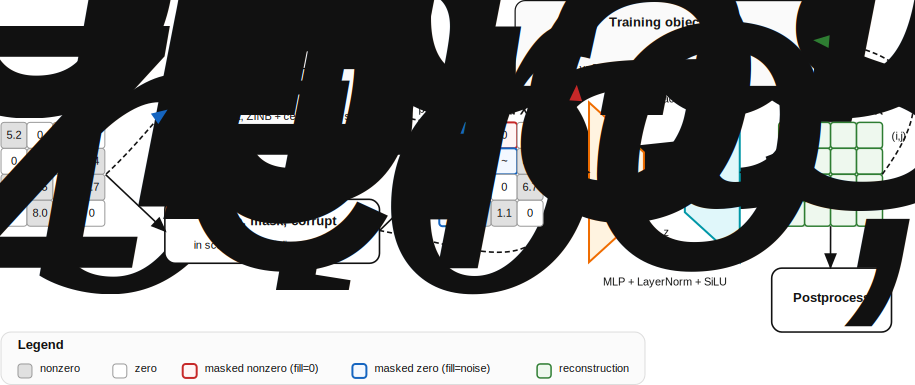
\includegraphics[width=\columnwidth]{figures/maskimpute_pipeline.png}
    \caption{\textbf{MaskClass overview.} Starting from logcounts
    $\mathbf{X}_{\log}$ and counts $\mathbf{C}$, we estimate a biozero
    probability $p_{\mathrm{bio}}(i,j)$ for observed zeros.
    During self-supervised training, non-zeros are masked at a fixed rate,
    while zeros are masked with probability proportional to $p_{\mathrm{bio}}$;
    masked zeros are corrupted by injecting noise and masked non-zeros are
    replaced by zero in the scaled space.
    A symmetric autoencoder reconstructs the scaled matrix, and parameters are
    learned by minimizing a weighted masked reconstruction loss plus an optional
    biozero regularizer (enabled in MaskClass$_{\mathrm{balanced}}$).}
    \label{fig:maskimpute_pipeline}
\end{figure}

\begin{algorithm}[H]
\caption{MaskClass training and imputation.}
\label{alg:maskclass}
\begin{algorithmic}[1]
\raggedright
\STATE \textbf{Input:} logcounts $\mathbf{X}_{\log}$, counts $\mathbf{C}$,
scaler $\mathrm{scale}/\mathrm{invscale}$, and hyperparameters
$p_{\mathrm{zero}},p_{\mathrm{nonzero}},\nu,\alpha,\gamma$, and epochs $E$.
\STATE Compute biozero probabilities $p_{\mathrm{bio}}(i,j)$ from counts
via the model in Section~\ref{sec:biozero}.
\STATE Compute $z_i=\frac{1}{G}\left|\{j: c_{ij}=0\}\right|$ and set
$p_{\mathrm{bio}}\leftarrow p_{\mathrm{bio}}(1-\alpha z_i)$.
\STATE Scale $\mathbf{S}\leftarrow\mathrm{scale}(\mathbf{X}_{\log})$.
\FOR{epoch $=1$ to $E$}
\FOR{mini-batch $\mathcal{B}$}
\STATE Sample $m_{ij}\sim\mathrm{Bernoulli}(\pi_{ij})$ where
$\pi_{ij}=p_{\mathrm{zero}}p_{\mathrm{bio}}(i,j)$ if $x_{ij}=0$ and
$\pi_{ij}=p_{\mathrm{nonzero}}$ if $x_{ij}>0$.
\STATE Corrupt inputs:
masked non-zeros $\tilde{s}_{ij}\leftarrow 0$; masked zeros
$\tilde{x}_{ij}=\log_2(1+\eta_{ij}c^{\max}_j)$ with
$\eta_{ij}\sim\mathrm{Uniform}(0,\nu)$ and $c^{\max}_j=\max_i c_{ij}$, then
$\tilde{s}_{ij}\leftarrow\mathrm{scale}(\tilde{x}_{ij})$.
\STATE Forward pass: $\hat{\mathbf{s}}_i=g_\phi(f_\theta(\tilde{\mathbf{s}}_i))$.
\STATE Minimize $\mathcal{L}=\mathcal{L}_{\mathrm{mask}}+\gamma\mathcal{L}_{\mathrm{bio}}$
(MaskClass$_{\mathrm{best}}$: $\gamma=0$; MaskClass$_{\mathrm{balanced}}$: $\gamma=1$).
\ENDFOR
\ENDFOR
\STATE Reconstruct $\mathbf{X}'_{\log}\leftarrow\mathrm{invscale}(\hat{\mathbf{S}})$ and keep observed non-zeros fixed.
\STATE \textbf{Output:} reconstructed logcounts $\mathbf{X}'_{\log}$.
\end{algorithmic}
\end{algorithm}
\FloatBarrier

  \subsection{Computational Considerations}
  The masked loss computes MSE only over masked entries, preventing trivial
  identity mapping. Robust scaling constrains dynamic range and stabilizes
  optimization, while inverse scaling restores original log‑count units for
  evaluation.

\section*{Software and Data}

If a paper is accepted, we strongly encourage the publication of software and
data with the camera-ready version of the paper whenever appropriate. This can
be done by including a URL in the camera-ready copy. However, \textbf{do not}
include URLs that reveal your institution or identity in your submission for
review. Instead, provide an anonymous URL or upload the material as
``Supplementary Material'' into the OpenReview reviewing system. Note that
reviewers are not required to look at this material when writing their review.

% Acknowledgements should only appear in the accepted version.
% \section*{Acknowledgements}

% \textbf{Do not} include acknowledgements in the initial version of the paper
% submitted for blind review.

% If a paper is accepted, the final camera-ready version can (and usually should)
% include acknowledgements.  Such acknowledgements should be placed at the end of
% the section, in an unnumbered section that does not count towards the paper
% page limit. Typically, this will include thanks to reviewers who gave useful
% comments, to colleagues who contributed to the ideas, and to funding agencies
% and corporate sponsors that provided financial support.

\section*{Impact Statement}
This paper presents work whose goal is to advance the field of Machine
Learning. There are many potential societal consequences of our work, none
which we feel must be specifically highlighted here.

\clearpage
\bibliography{references}
\bibliographystyle{icml2026}
\end{document}
